\documentclass[conference]{IEEEtran}
\IEEEoverridecommandlockouts

\usepackage{fontspec}
\setmainfont{texgyretermes-regular.otf}[BoldFont=texgyretermes-bold.otf, ItalicFont=texgyretermes-italic.otf, BoldItalicFont=texgyretermes-bolditalic.otf]
\setsansfont{texgyreheros-regular.otf}[BoldFont=texgyreheros-bold.otf, ItalicFont=texgyreheros-italic.otf]
\setmonofont{texgyrecursor-regular.otf}[BoldFont=texgyrecursor-bold.otf]
\usepackage[spanish,es-noquoting]{babel}
\usepackage{amsmath,amssymb}
\usepackage{graphicx}
\usepackage{booktabs}
\usepackage{url}
\usepackage[hidelinks]{hyperref}

\graphicspath{{../reports/figures/}}

\def\BibTeX{{\rm B\kern-.05em{\sc i\kern-.025em b}\kern-.08em T\kern-.1667em\lower.7ex\hbox{E}\kern-.125emX}}

\begin{document}

\title{Dinámica de la marcha para el diagnóstico diferencial\\de enfermedades neurodegenerativas:\\análisis exploratorio y riesgos metodológicos}

\author{
\IEEEauthorblockN{Luis Renato Alvarez Ccopa, Andersson Chiroque Silva \\ David Teofilo Orihuela Serafin, Jeraldine Dione Rojas Vargas}
\IEEEauthorblockA{\textit{Universidad de Ingeniería y Tecnología} \\
Lima, Perú}
}

\maketitle

\begin{abstract}
El Parkinson, la enfermedad de Huntington y la esclerosis lateral amiotrófica (ELA) alteran el control motor por mecanismos distintos y producen patrones de marcha distinguibles. Este trabajo plantea el diagnóstico diferencial entre las tres patologías y sujetos sanos como un problema de clasificación multiclase sobre descriptores derivados de series temporales de zancada, usando la base \textit{Gait in Neurodegenerative Disease} de PhysioNet (64 sujetos, 15\,160 zancadas). Esta primera entrega presenta la formulación del problema y el análisis exploratorio de los datos. Se documentan cuatro defectos de la metadata clínica que impiden su carga directa, incluida una fuga de la variable objetivo a través de la columna de severidad. Se muestra que las series se distribuyen sin filtrar y que la decisión de filtrado no ajusta los resultados sino que los determina: sin filtrar, el grupo con ELA aparenta la marcha más inestable (coeficiente de variación de 0.43, diez veces el de los controles), mientras que tras aplicar reglas de validez fisiológica ese valor cae a 0.063 y el grupo más inestable pasa a ser Huntington (0.105), en concordancia con la fisiopatología coreica. Se cuantifica además la fuga de información por sujeto: particionar aleatoriamente ventanas de zancadas en lugar de agrupar por individuo infla la exactitud balanceada de 0.62 a 0.81 con los mismos datos y el mismo modelo. Por último se identifica un confusor demográfico no corregible en la cohorte principal --- los controles son 27 años más jóvenes que los pacientes con Parkinson --- y se incorpora una segunda cohorte de 165 sujetos cuyos grupos sí están pareados por edad, que permitirá aislar ese efecto. Estos hallazgos fijan los requisitos metodológicos de la segunda entrega.
\end{abstract}

\begin{IEEEkeywords}
análisis de marcha, enfermedades neurodegenerativas, clasificación multiclase, fuga de información, análisis exploratorio de datos
\end{IEEEkeywords}

\section{Introducción y formulación del problema}

\subsection{Motivación}

Las enfermedades neurodegenerativas deterioran el control motor por vías distintas. La enfermedad de Parkinson degrada la vía dopaminérgica de los ganglios basales y produce bradicinesia, rigidez y una marcha de pasos cortos. La enfermedad de Huntington genera movimientos coreicos involuntarios que vuelven la marcha errática e impredecible. La esclerosis lateral amiotrófica ataca la motoneurona y produce debilidad progresiva que obliga a estrategias compensatorias de estabilidad. Las tres alteran la forma de caminar, pero no de la misma manera.

El diagnóstico diferencial temprano entre estas patologías es clínicamente difícil y descansa en gran medida en la evaluación subjetiva de especialistas. Una marcha instrumentada de cinco minutos con sensores de fuerza en el calzado es barata, no invasiva y repetible, lo que la convierte en un candidato atractivo para apoyar la decisión clínica. El trabajo seminal de Hausdorff et al.\ estableció que la dinámica del intervalo de zancada contiene marcadores cuantitativos de patología: la variabilidad aumenta y las correlaciones de largo alcance se reducen en Huntington \cite{hausdorff1997} y en ELA \cite{hausdorff2000}. Una revisión reciente del área documenta un volumen creciente de trabajo sobre estos mismos datos \cite{gaitsurvey2024}.

\subsection{Tarea de Machine Learning}

El problema se formula como \textbf{clasificación supervisada multiclase} con el sujeto como unidad de análisis. Dada una serie temporal de intervalos de zancada de aproximadamente 250 observaciones, el objetivo es asignar al sujeto a una de cuatro clases: control sano, Parkinson, Huntington o ELA. El conjunto tiene 64 sujetos con clases desbalanceadas, por lo que se adoptan la exactitud balanceada y el $F_1$ macro como métricas principales.

\subsection{Preguntas de investigación}

\textbf{PI1.} ¿La dinámica temporal de la marcha permite discriminar \emph{entre} enfermedades neurodegenerativas, o únicamente separar enfermos de sanos?

\textbf{PI2.} ¿Qué magnitud de sesgo optimista introduce evaluar a nivel de zancada en lugar de a nivel de sujeto? Esta decisión metodológica es frecuente en la literatura que usa este conjunto de datos y su efecto no suele cuantificarse.

\textbf{PI3.} ¿La señal discriminante es atribuible a la patología, o la explican confusores demográficos y de protocolo, en particular la edad, el sexo y la velocidad de marcha?

\section{Datos}

\subsection{Origen y protocolo}

Los datos provienen de la base \textit{Gait in Neurodegenerative Disease Database} \cite{hausdorff2000}, distribuida en PhysioNet \cite{goldberger2000} bajo licencia Open Data Commons Attribution v1.0, de acceso abierto y sin requisitos de registro.

Cada uno de los 64 participantes caminó durante cinco minutos a paso cómodo por un pasillo de 77 metros, con resistores sensibles a la fuerza colocados bajo cada pie. La señal se digitalizó a 300\,Hz, lo que da 90\,000 muestras por canal. Los 64 registros comparten exactamente la misma duración y frecuencia de muestreo, de modo que el protocolo de captura no introduce variabilidad que controlar.

\subsection{Estructura}

El conjunto tiene tres niveles de información por sujeto: la señal cruda de fuerza de cada pie, una serie derivada con trece medidas temporales por zancada (intervalos de zancada, balanceo, apoyo y apoyo doble, en segundos y como porcentaje del ciclo) y una tabla de metadata clínica con edad, sexo, talla, peso, velocidad de marcha y severidad. El análisis trabaja sobre el nivel derivado, que totaliza 15\,160 zancadas.

\begin{table}[t]
\caption{Composición de la cohorte}
\label{tab:cohorte}
\centering
\begin{tabular}{lrrrrr}
\toprule
Grupo & $n$ & Edad & \% hombres & Velocidad & Zancadas \\
 & & (años) & & (m/s) & \\
\midrule
Control    & 16 & 39.3 & 12.5 & 1.35 & 4\,076 \\
Parkinson  & 15 & 66.8 & 66.7 & 1.00 & 3\,688 \\
Huntington & 20 & 46.7 & 30.0 & 1.15 & 4\,846 \\
ELA        & 13 & 55.6 & 76.9 & 1.05 & 2\,550 \\
\midrule
Total      & 64 & 48.4 & 40.6 & 1.16 & 15\,160 \\
\bottomrule
\end{tabular}
\end{table}

\subsection{Cohorte de validación externa}

Como cohorte independiente se incorpora la base \textit{Gait in Parkinson's Disease} \cite{frenkel2005}, con 93 pacientes con Parkinson y 73 controles registrados con un protocolo distinto: ocho sensores de fuerza bajo cada pie a 100\,Hz durante aproximadamente dos minutos. Reúne tres estudios con protocolos diferentes --- doble tarea, estimulación auditiva rítmica y caminadora --- de modo que el estudio de origen constituye un confusor de protocolo adicional.

Su valor para este trabajo excede la simple comprobación de generalización. Como muestra la Tabla~\ref{tab:pareamiento}, sus grupos están \textbf{pareados por edad}: la diferencia entre pacientes y controles es de 2.6 años y no alcanza significancia estadística, frente a los 27.5 años de la cohorte principal. El desbalance por sexo también desaparece (54.8\,\% de hombres en controles contra 62.4\,\% en pacientes, frente a 12.5\,\% contra 66.7\,\% en \texttt{gaitndd}). Esto la convierte en el instrumento para aislar el efecto del confusor demográfico descrito en la Sección~\ref{sec:confusores}: si el eje Parkinson--control se sostiene en una cohorte donde la edad no discrimina, la edad no era el mecanismo.

\begin{table}[t]
\caption{Pareamiento por edad en ambas cohortes (prueba de Welch)}
\label{tab:pareamiento}
\centering
\begin{tabular}{lrrrr}
\toprule
Cohorte & Control & Parkinson & Dif. & $p$ \\
 & (años) & (años) & & \\
\midrule
\texttt{gaitndd} & 39.3 ($n$=16) & 66.8 ($n$=15) & $+27.5$ & $3.2\times10^{-5}$ \\
\texttt{gaitpdb} & 63.7 ($n$=73) & 66.3 ($n$=93) & $+2.6$ & $0.063$ \\
\bottomrule
\end{tabular}
\end{table}

Esta cohorte presenta sus propios defectos de formato, documentados en el repositorio: las filas de su tabla demográfica terminan con un número variable de tabuladores de relleno, lo que hace fallar la lectura tabulada estándar; el estudio \texttt{Ju} registra la talla en centímetros mientras los otros dos la registran en metros, de manera que sin normalizar la columna identifica el estudio de origen; y una fila con identificador mal escrito (\texttt{Juc010} por \texttt{JuCo10}) corresponde a un sujeto sin archivos de señal, por lo que de los 166 sujetos declarados solo 165 tienen datos. Sus puntajes UPDRS y de estadio Hoehn \& Yahr \cite{hoehn1967} separan los grupos de forma perfecta --- el estadio vale 0 en todos los controles y entre 2 y 3 en todos los pacientes --- por lo que son fuga de la etiqueta como predictores y se reservan para la tarea secundaria de regresión de severidad dentro del grupo de pacientes.

Finalmente, sus 306 grabaciones provienen de 165 sujetos, con hasta siete caminatas por paciente en el estudio \texttt{Ju}. La estructura de repetición reproduce el problema de fuga de la Sección~\ref{sec:fuga} y obliga al mismo particionamiento agrupado.

\section{Análisis exploratorio de datos}

\subsection{La metadata clínica exige un parser propio}

El archivo de descripción de sujetos presenta cuatro defectos que impiden su carga directa.

\textbf{Un salto de línea parte un registro.} La fila del sujeto \texttt{hunt20} está dividida en dos líneas, de modo que una lectura tabulada estándar devuelve 65 filas para 64 sujetos y convierte a ese individuo en dos observaciones corruptas.

\textbf{Los faltantes son una cadena literal.} Cuatro campos se codifican como el texto \texttt{MISSING}: la velocidad de marcha de \texttt{hunt20}, \texttt{als4} y \texttt{als5}, y el peso de \texttt{als13}. Al leerse como texto, las columnas afectadas dejan silenciosamente de ser numéricas.

\textbf{La variable objetivo declarada está mal.} Los trece sujetos con ELA tienen el valor \texttt{subjects} en la columna de grupo, no \texttt{als}. Usar esa columna como etiqueta produce una clase espuria y elimina la clase ELA. La etiqueta confiable es el prefijo del identificador del registro.

\textbf{Una columna contiene cuatro escalas incomparables.} El campo de severidad almacena el estadio Hoehn \& Yahr en Parkinson (1.5--4, donde más es peor), la capacidad funcional total en Huntington \cite{shoulson1979} (1--12, donde \emph{menos} es peor), los meses desde el diagnóstico en ELA (1--54) y un cero de relleno en los controles. Además de ser semánticamente inconsistente, el rango de valores identifica el grupo casi perfectamente, por lo que constituye una \textbf{fuga de la variable objetivo} \cite{kaufman2012} y queda excluida del modelado.

\subsection{Confusores en la composición de la cohorte}
\label{sec:confusores}

La Tabla~\ref{tab:cohorte} y la Fig.~\ref{fig:confusores} muestran que los cuatro grupos no son comparables entre sí. Los controles promedian 39.3 años y los pacientes con Parkinson 66.8: una diferencia de 27 años. La composición por sexo va de 12.5\,\% de hombres en controles a 76.9\,\% en ELA. Un clasificador entrenado sobre descriptores correlacionados con la edad o el sexo podría separar los grupos sin aprender nada sobre la patología.

La velocidad de marcha admite una lectura distinta: la lentitud es consecuencia de la enfermedad y no un artefacto de muestreo. Sin embargo, determina mecánicamente buena parte de los descriptores temporales, lo que obliga a verificar si la señal discriminante sobrevive a su control.

\begin{figure*}[t]
\centering
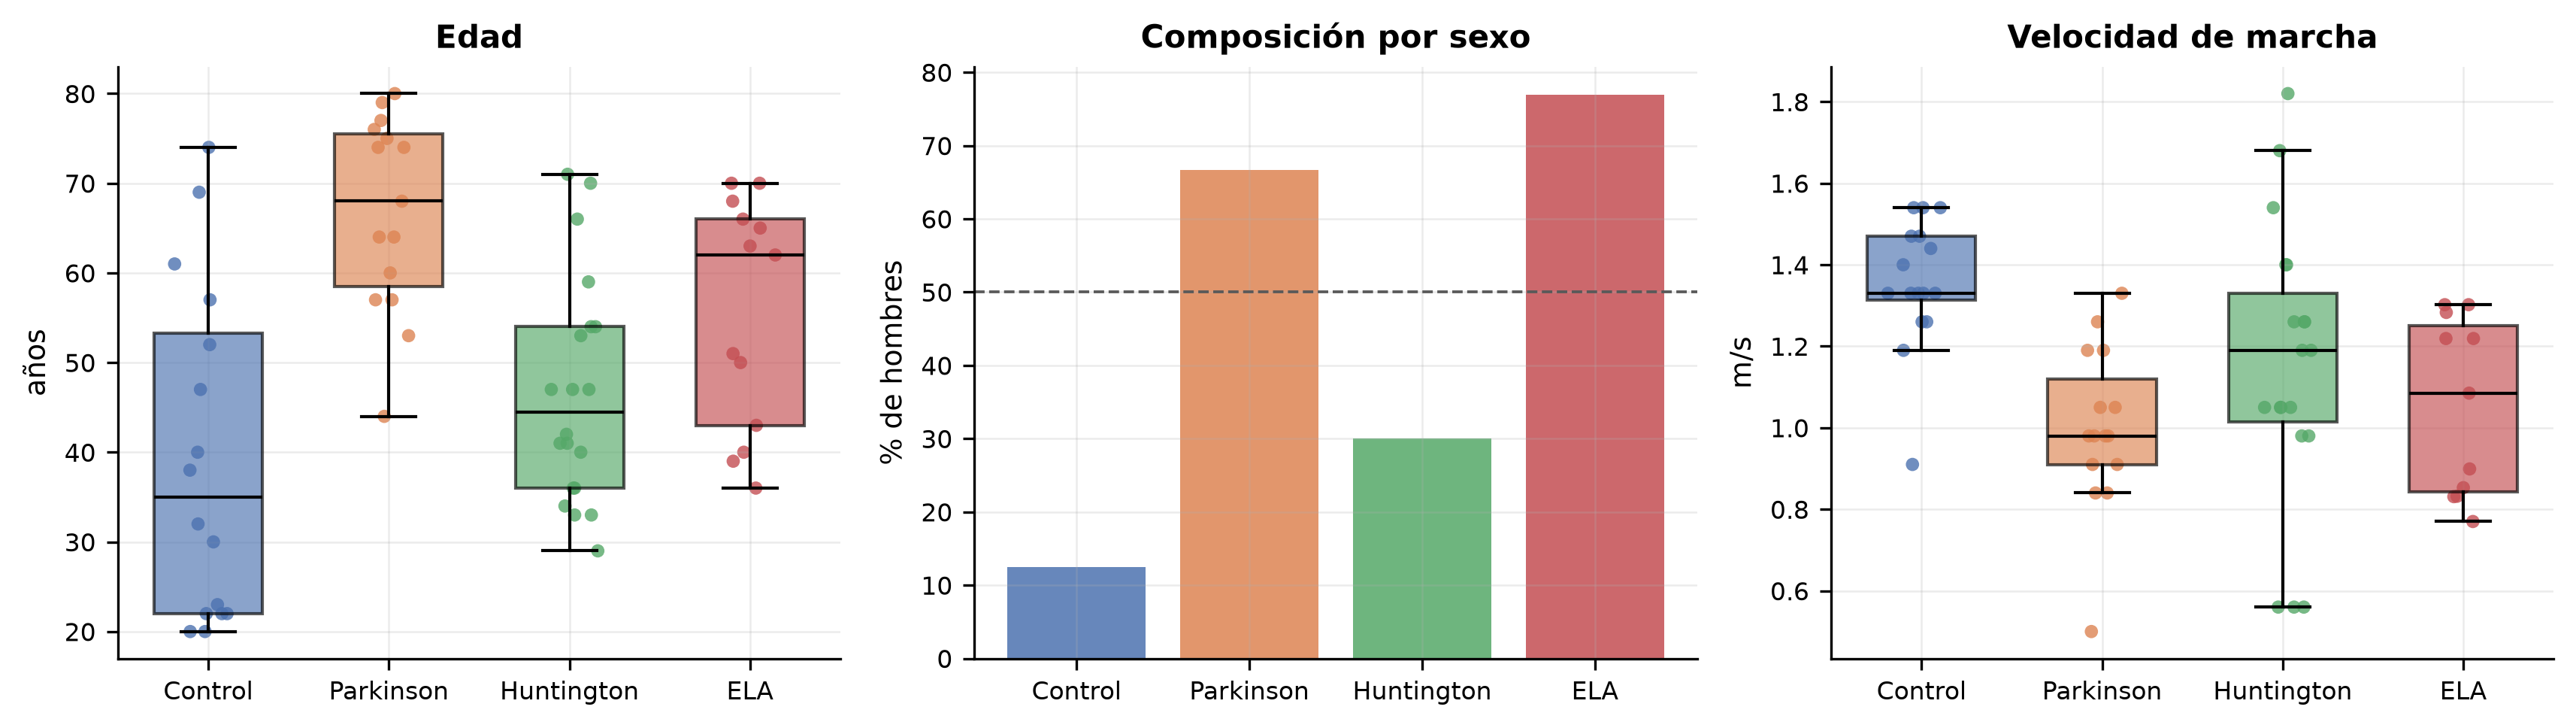
\includegraphics[width=0.86\textwidth]{confusores_demograficos.png}
\caption{Distribución de edad, composición por sexo y velocidad de marcha por grupo. El grupo control es marcadamente más joven y mayoritariamente femenino frente a las cohortes patológicas.}
\label{fig:confusores}
\end{figure*}

Un indicio adicional de que las cohortes se recolectaron por separado aparece en la talla declarada: la media de las mujeres del grupo control es 1.82\,m y la de Huntington 1.79\,m, valores implausibles, mientras que el grupo ELA reporta 1.66\,m y usa tres decimales con la firma de una conversión desde unidades imperiales. Talla y peso se excluyen del modelado por no ser comparables entre grupos.

\subsection{Calidad de las series temporales}

La documentación oficial advierte que las series derivadas no están filtradas. En efecto contienen intervalos de zancada de hasta 55 segundos, producto de pausas, giros al final del pasillo o pisadas no detectadas.

Se definieron tres reglas de validez, todas derivadas de restricciones físicas y no de criterios estadísticos: el intervalo de zancada debe estar entre 0.5 y 2.5\,s; el tiempo de apoyo doble no puede ser negativo; y las fases expresadas como porcentaje del ciclo deben permanecer en $[0, 100]$. Una cuarta comprobación, que las fases de balanceo y apoyo sumen 100\,\%, se satisface en las 15\,160 zancadas: la derivación interna es aritméticamente consistente y los problemas provienen de la detección de pisadas.

Las reglas descartan el 2.8\,\% de las zancadas, con una incidencia muy desigual entre grupos: 5.9\,\% en ELA y 5.4\,\% en Huntington frente a 0.02\,\% en controles.

\textbf{Un registro resulta inutilizable.} El sujeto \texttt{hunt20} viola alguna regla en el 100\,\% de sus zancadas. Su intervalo de zancada mediano del pie derecho es de 42.9\,s contra 0.99\,s del izquierdo; la fase de apoyo derecha ocupa el 98\,\% del ciclo cuando lo normal es cerca del 60\,\%, y el apoyo doble resultante varía entre $-70$\,\% y $+4317$\,\%. El canal derecho no registró despegues. Sumado a que su registro comienza 42 segundos tarde, a que su velocidad de marcha es un faltante y a que es el sujeto cuya fila está partida en la metadata, el registro se excluye. El análisis continúa con 63 sujetos.

\subsection{El filtrado determina las conclusiones}

El coeficiente de variación del intervalo de zancada es el marcador clásico de inestabilidad de la marcha. La Tabla~\ref{tab:filtrado} lo calcula antes y después de aplicar las reglas de validez.

\begin{table}[t]
\caption{Coeficiente de variación del intervalo de zancada antes y después del filtrado de artefactos}
\label{tab:filtrado}
\centering
\begin{tabular}{lrrr}
\toprule
Grupo & Sin filtrar & Filtrado & Factor \\
\midrule
Control    & 0.044 & 0.041 & 1.08 \\
Parkinson  & 0.189 & 0.074 & 2.56 \\
Huntington & 0.138 & 0.105 & 1.32 \\
ELA        & 0.431 & 0.063 & 6.80 \\
\bottomrule
\end{tabular}
\end{table}

Sin filtrar, el grupo con ELA exhibe una variabilidad diez veces superior a la de los controles y cualquier lectura concluiría que la ELA produce la marcha más inestable de las tres patologías. Tras descartar el 5.9\,\% de zancadas inválidas del grupo --- 23 de ellas fuera de todo rango fisiológico, con duraciones de hasta 55 segundos --- el coeficiente cae a 0.063, apenas un 50\,\% por encima del control. La variabilidad aparente era casi enteramente artefacto de medición.

Con los datos filtrados el orden se invierte y el grupo más inestable pasa a ser Huntington, lo que sí concuerda con la fisiopatología coreica y con los hallazgos originales de Hausdorff et al.\ \cite{hausdorff1997}. En este conjunto de datos, la decisión de filtrado no ajusta los resultados: los determina.

Esta decisión tiene un costo que conviene declarar. El filtrado es diferencial por clase --- elimina 260 zancadas en Huntington y solo 1 en controles --- y necesariamente lo es, porque la marcha patológica genera más fallos de detección. Queda abierto si una zancada de tres segundos en un paciente con Huntington es un error del sensor o un episodio de congelamiento real. Por eso se adopta un criterio conservador: se aplican únicamente el rango fisiológico y las reglas de consistencia interna, y no un filtro por dispersión robusta que descartaría otras 324 zancadas por ser estadísticamente atípicas y borraría variabilidad potencialmente real.

\subsection{Descriptores y separabilidad (PI1)}

De cada serie filtrada se extraen descriptores de cuatro familias: ritmo (duración media de zancada, cadencia), dispersión (desviación estándar, coeficiente de variación, rango intercuartílico), simetría entre lados y estructura temporal. Esta última incluye la autocorrelación de retardo uno y el exponente $\alpha$ de \textit{detrended fluctuation analysis} \cite{peng1995}, que mide si las fluctuaciones del intervalo de zancada mantienen correlación a largo plazo; un valor cercano a 0.5 indica que la serie degeneró en ruido blanco.

\begin{table}[t]
\caption{Descriptores por grupo tras el filtrado (media por sujeto)}
\label{tab:descriptores}
\centering
\begin{tabular}{lrrrr}
\toprule
Grupo & Zancada & CV & Apoyo doble & $\alpha$ \\
 & (s) & & (\% ciclo) & (DFA) \\
\midrule
Control    & 1.097 & 0.041 & 28.2 & 0.875 \\
Parkinson  & 1.125 & 0.074 & 34.0 & 0.805 \\
Huntington & 1.152 & 0.105 & 32.0 & 0.653 \\
ELA        & 1.356 & 0.063 & 35.3 & 0.850 \\
\bottomrule
\end{tabular}
\end{table}

Los descriptores se ordenan de manera coherente con la clínica de cada patología (Tabla~\ref{tab:descriptores}, Fig.~\ref{fig:descriptores}). Huntington pierde estructura temporal: su $\alpha$ cae a 0.65 y su autocorrelación de retardo uno a 0.19, frente a 0.88 y 0.49 en controles. Su marcha no solo es más variable, sino variable sin memoria, lo esperable de un control motor desregulado por corea. La ELA presenta la zancada más larga y el mayor porcentaje de apoyo doble, patrón compensatorio ante debilidad muscular progresiva. El Parkinson ocupa una posición intermedia en casi todos los descriptores, lo que anticipa que será la clase más difícil de separar.

Ningún descriptor aislado separa las cuatro clases. La respuesta preliminar a PI1 es que existe señal discriminante, pero es multivariada y parcial.

\begin{figure*}[t]
\centering
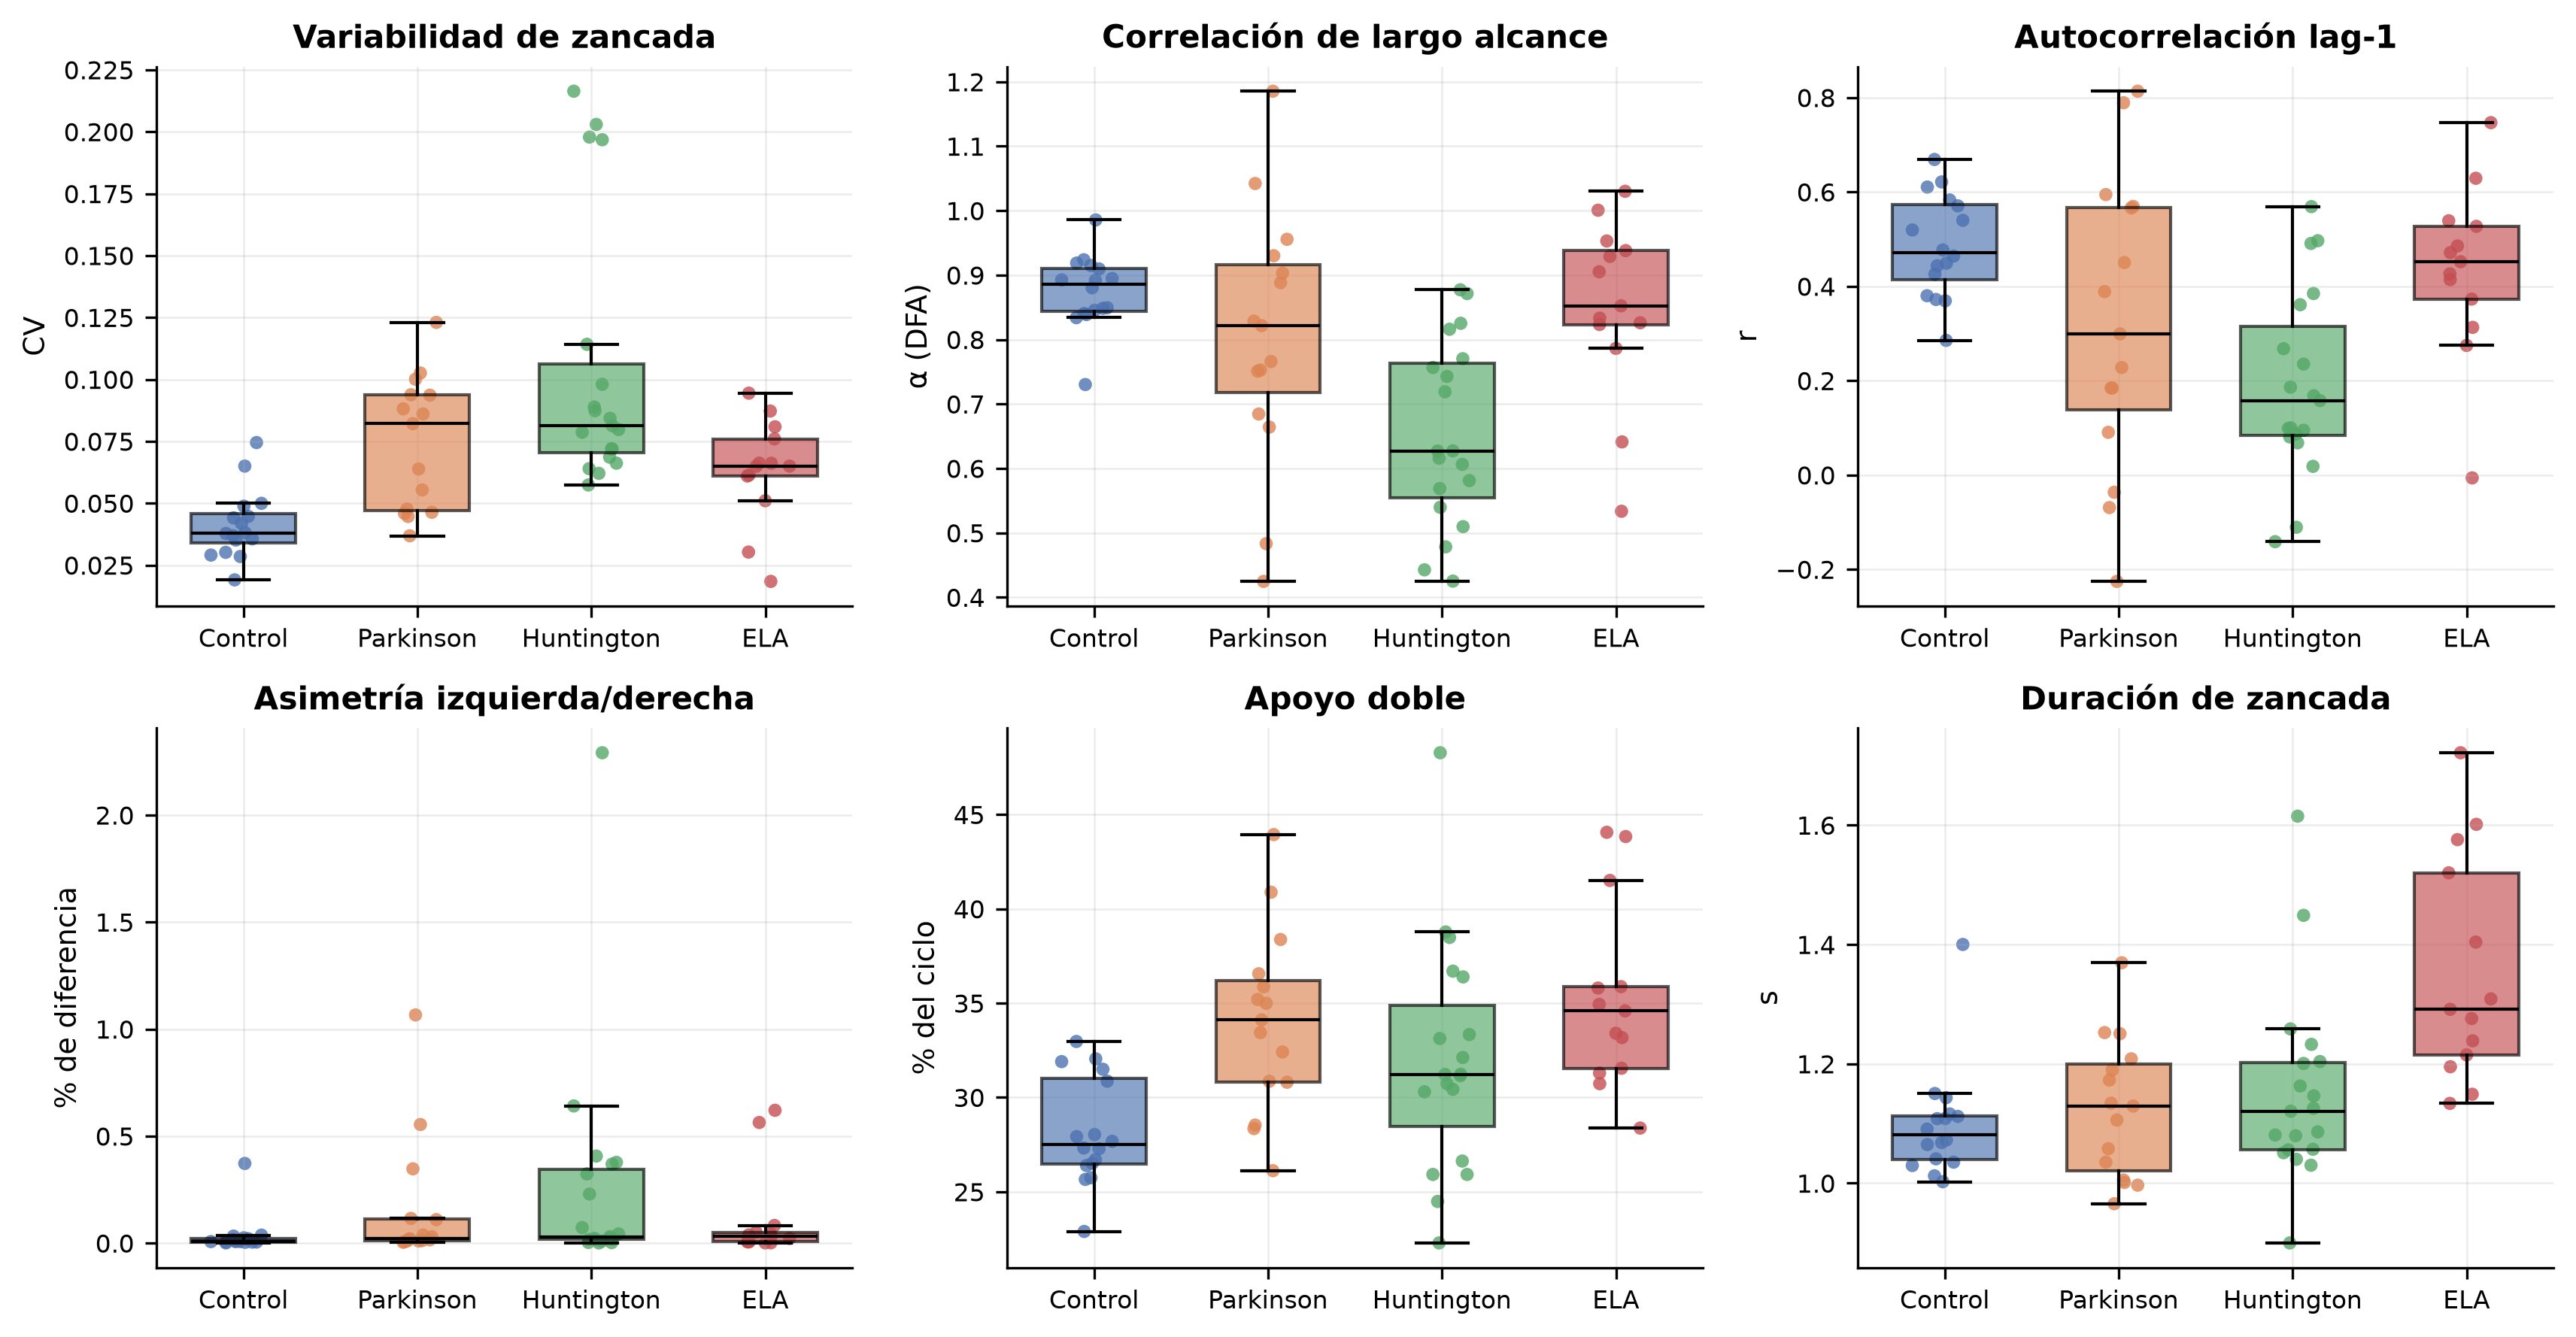
\includegraphics[width=0.92\textwidth]{descriptores_por_grupo.png}
\caption{Distribución por grupo de seis descriptores de marcha tras el filtrado de artefactos. Cada punto es un sujeto. Todas las distribuciones se solapan: ningún descriptor aislado separa las cuatro clases.}
\label{fig:descriptores}
\end{figure*}

\subsection{Descriptores frente a confusores (PI3)}

La velocidad de marcha correlaciona con todos los descriptores: $-0.64$ con el porcentaje de apoyo doble, $-0.53$ con la variabilidad y $-0.48$ con la duración de zancada. Parte de esa relación es mecánica. Sin embargo, al examinar la relación dentro de cada grupo, la pendiente entre velocidad y variabilidad es aproximadamente plana: la velocidad separa los grupos porque los pacientes caminan más lento, pero no explica la variabilidad dentro de un grupo. La edad presenta correlaciones más débiles, con un máximo de 0.37.

La conclusión sobre PI3 es cautelosa dentro de la cohorte principal. La edad y el sexo no son controlables con su diseño, porque el grupo control es 27 años más joven y mayoritariamente femenino, de modo que cualquier desempeño que se reporte sobre ella incorpora una componente demográfica inseparable. La respuesta definitiva a PI3 se obtendrá en la segunda entrega comparando el desempeño del eje Parkinson--control entre esta cohorte y la cohorte pareada de la Tabla~\ref{tab:pareamiento}.

\subsection{Fuga de información por sujeto (PI2)}
\label{sec:fuga}

Sesenta y tres sujetos son pocos para entrenar. La práctica habitual en la literatura sobre estos datos consiste en trocear la serie de cada sujeto en ventanas y tratar cada ventana como una observación independiente, lo que multiplica las filas por un factor cercano a ocho. Pero las ventanas de un mismo sujeto comparten fisiología, calzado, sesión y antropometría: no son independientes. Una partición aleatoria permite que el modelo reconozca al individuo en lugar de la enfermedad \cite{saeb2017}.

\begin{table}[t]
\caption{Exactitud balanceada según la unidad de análisis y la estrategia de partición, con el mismo modelo (bosque aleatorio, 300 árboles) y los mismos descriptores}
\label{tab:leakage}
\centering
\begin{tabular}{llrr}
\toprule
Unidad & Partición & $n$ & Exactitud bal. \\
\midrule
Ventana de 30 zancadas & Aleatoria      & 482 & $0.812 \pm 0.049$ \\
Ventana de 30 zancadas & Por sujeto     & 482 & $0.622 \pm 0.086$ \\
Sujeto                 & Estratificada  & 63  & $0.642 \pm 0.048$ \\
\bottomrule
\end{tabular}
\end{table}

La Tabla~\ref{tab:leakage} cuantifica el efecto. La partición aleatoria infla la exactitud balanceada en 19 puntos porcentuales con exactamente los mismos datos, descriptores y modelo. La verificación decisiva está en la tercera fila: evaluar directamente a nivel de sujeto, sin ventanas y sin posibilidad de fuga, produce 0.642, un valor que coincide con la estimación agrupada y no con la aleatoria. Esto confirma que la partición agrupada es el estimador correcto y que la diferencia es optimismo puro, no una ventaja real de disponer de más filas. Como referencia, el azar en cuatro clases equilibradas daría 0.25, de modo que existe señal real, aunque considerablemente menor que la sugerida por la cifra inflada.

\section{Siguientes pasos}

Los hallazgos anteriores fijan los requisitos de la segunda entrega.

\textbf{Protocolo de evaluación.} Toda validación agrupará por sujeto mediante validación cruzada estratificada por grupos o \textit{leave-one-subject-out}, con búsqueda de hiperparámetros anidada dentro del bucle de validación para no reintroducir la fuga por otra puerta. Dado el tamaño muestral reducido, los resultados se reportarán con intervalos de confianza por remuestreo sobre sujetos \cite{varoquaux2018}.

\textbf{Baselines.} Se establecerán dos referencias: un clasificador trivial por clase mayoritaria y un baseline clínico que use únicamente la velocidad de marcha. Si los descriptores de dinámica temporal no superan a la velocidad por sí sola, no justifican su complejidad.

\textbf{Modelos.} Se compararán al menos dos familias sobre los descriptores por sujeto --- regresión logística multinomial regularizada y un ensamble de árboles --- junto con una red convolucional unidimensional sobre la serie cruda de intervalos como tercer enfoque. La implementación se apoyará en scikit-learn \cite{pedregosa2011}.

\textbf{Validación externa.} El eje Parkinson--control se evaluará sobre la cohorte independiente \cite{frenkel2005}, capturada con otro protocolo, para estimar la generalización fuera de la cohorte de entrenamiento.

\textbf{Análisis de confusores.} El eje Parkinson--control se entrenará y evaluará por separado en la cohorte confundida y en la cohorte pareada por edad. La diferencia de desempeño entre ambas acota el efecto demográfico. Complementariamente se reentrenará restringiendo la cohorte principal a subgrupos comparables por edad.

\textbf{Interpretación.} Se analizarán la importancia por permutación agrupada por sujeto y la matriz de confusión, con atención particular a la separación Parkinson--ELA, que los descriptores anticipan como la más problemática.

\section{Conclusiones preliminares}

El análisis exploratorio establece que el conjunto de datos contiene señal discriminante real entre las cuatro clases, pero que su explotación honesta exige decisiones metodológicas que la literatura del área no siempre hace explícitas. Tres resultados concentran el aporte de esta entrega: la metadata clínica contiene una fuga de la variable objetivo y cuatro defectos de formato que invalidan una carga directa; el filtrado de artefactos de medición invierte cuál es el grupo con la marcha más inestable; y la partición por zancada en lugar de por sujeto infla la exactitud balanceada en 19 puntos porcentuales. La segunda entrega desarrollará el modelado bajo los requisitos que estos hallazgos imponen.

\section*{Disponibilidad del código}

El código, los notebooks y las instrucciones de reproducción están disponibles en el repositorio público del proyecto. Los datos se descargan desde PhysioNet mediante el código incluido y no se redistribuyen.

\bibliographystyle{IEEEtran}
\bibliography{refs}

\end{document}
